\section{Implementation}
We implement our tool in JavaScript because we want our tool to be a web-based application, which can be easy to access. JavaScript also has a library called D3.js that is used for producing data visualization in web browsers. Our tool can be run in web browsers. We use the built-in HTTP server , \texttt{SimpleHTTPServer}, to test and run our tool. Next we describe UI components and other tools we use in order to implement our web-based application.
\subsection{UI Components}
Our tool consists of multiple UI components as follows:
\begin{itemize}
	\item \textbf{World Map Layer}: we use the geojson data~\cite{geocountries}, which contains information for each country, such as country polygon coordinates to draw the world map and ISO ALPHA-3 code.
	\item \textbf{HDI Map layer}: HDI Map layer is built on top of World Map Layer, where we color each country polygon with a unique color based on how high its HDI is. As shown in Figure~\ref{fig:hdi}, the countries with high HDI value are colored bluish while the countries with low HDI value are colored reddish.
	\begin{figure}[t]
        \centering
		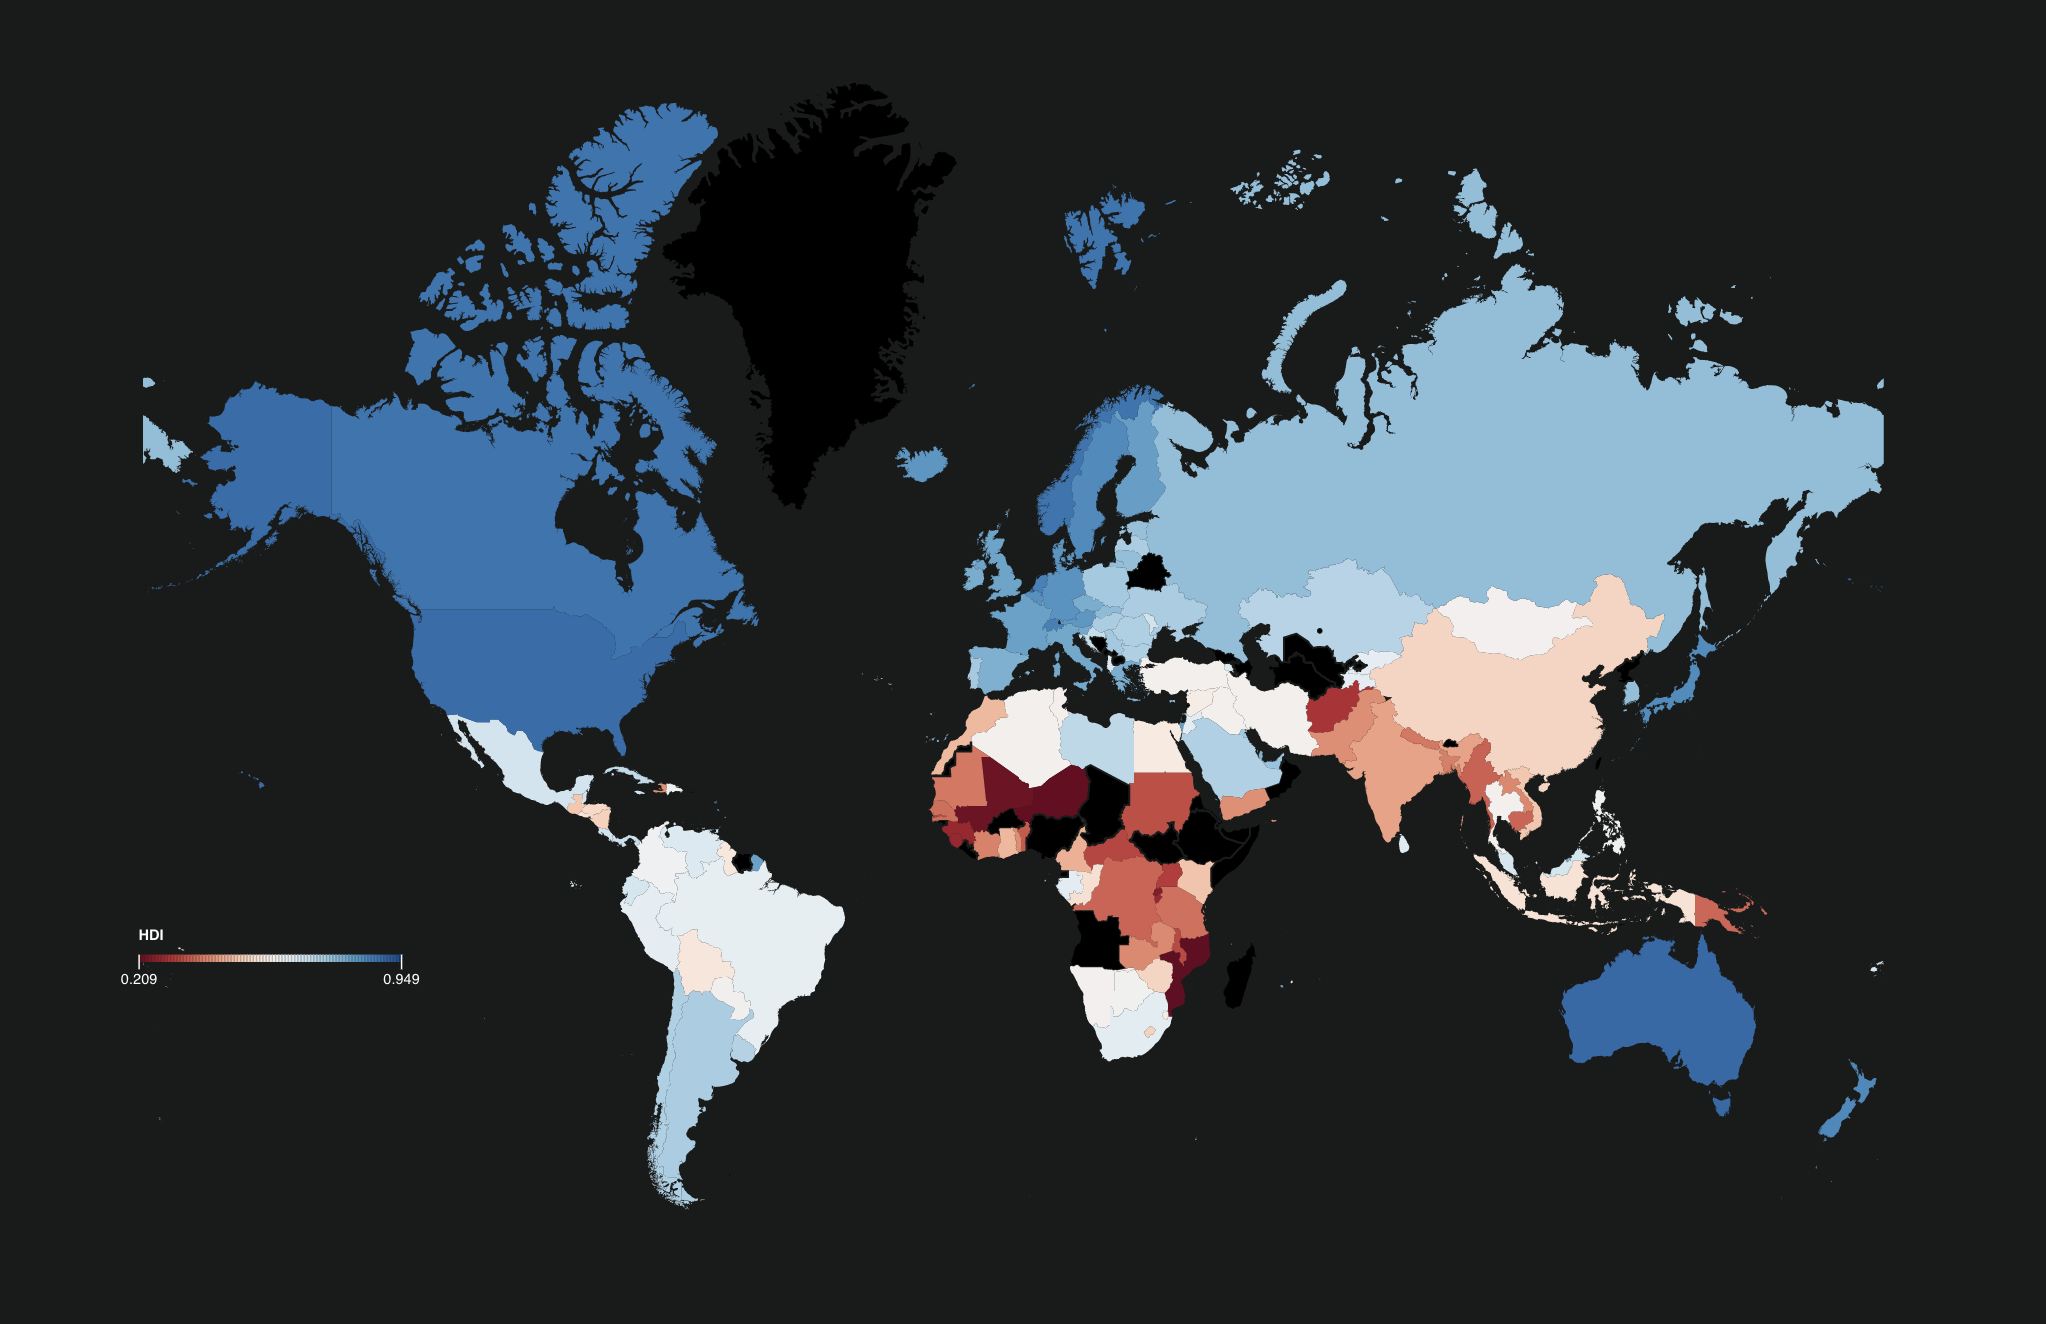
\includegraphics[width=0.4\textwidth]{hdiMap}
		\caption{HDI Map Layer}
		\label{fig:hdi}
	\end{figure}
	\item \textbf{Bivariate Map Layer}: Bivariate Map Layer shows a bivariate map. The legends of bivariate map have two axises. Each axis consists of three gradual colors, so there are nine combined colors in total. In our case, Bivariate Map Layer is used to compare two components of HDI and helps users any possible correlation between the two components. For example, Figure \ref{fig:bivariate} shows that most of the countries in the world have low values of GNI with high expected years of schooling.
	\begin{figure}[t]
        \centering
		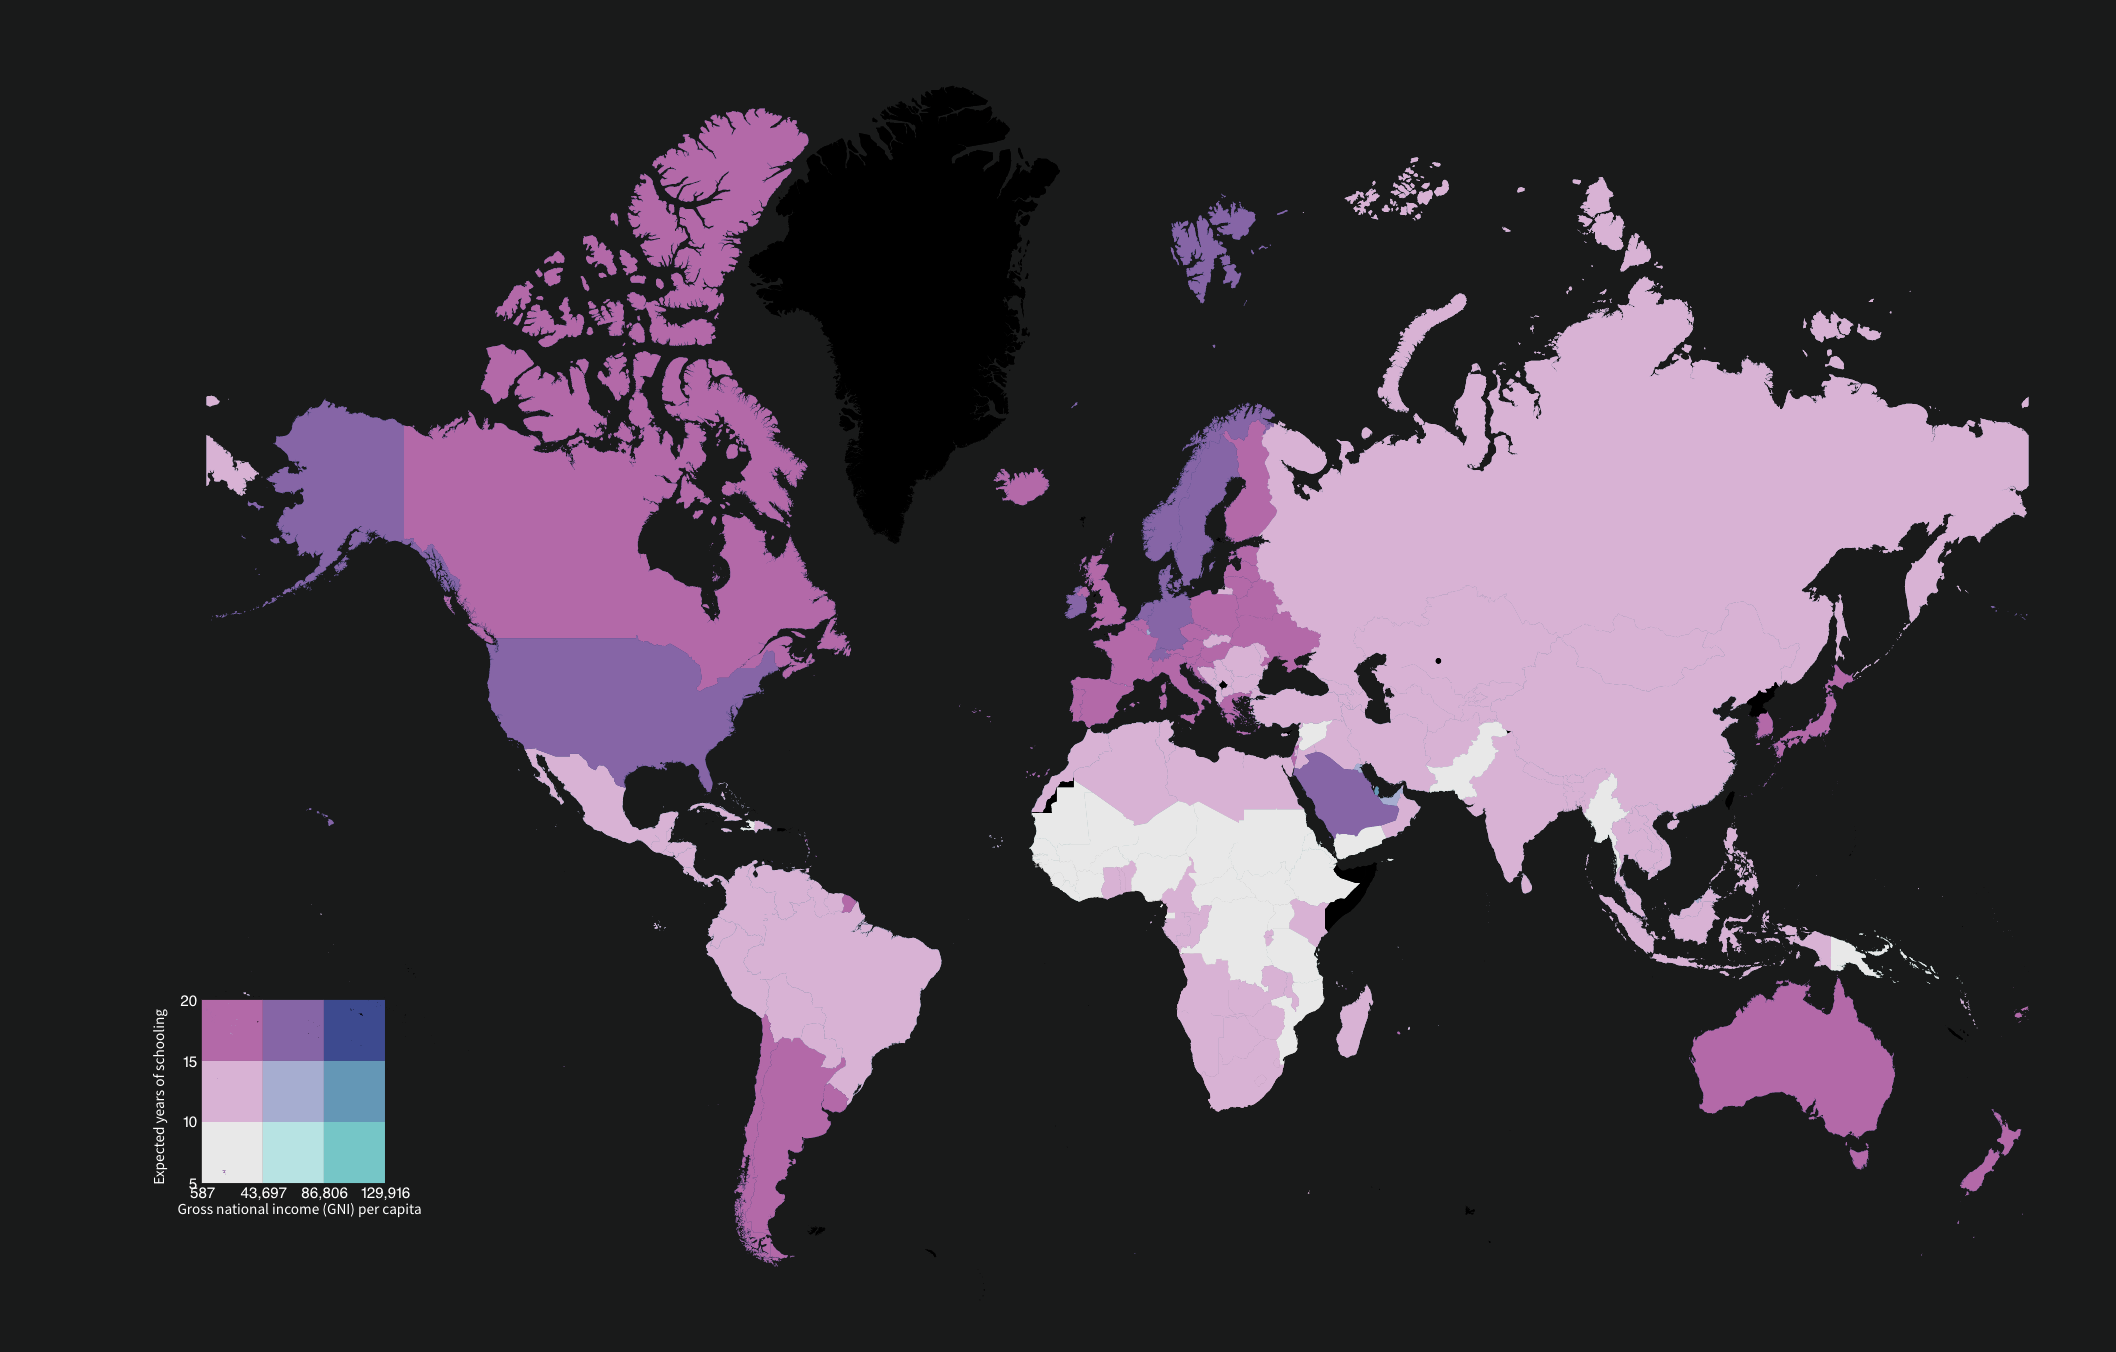
\includegraphics[width=0.4\textwidth]{bivariateMap}
		\caption{Bivaraite Map Layer}
		\label{fig:bivariate}
	\end{figure}
	\item \textbf{Parallel Coordinate Plot:} we use the parallel coordinate plot to show the values of HDI along with its components for all the countries. Each vertical axis represents a component. Thus, each line in the plot represents a country. We allow users to brush on each vertical axis to select a range of values they are interested in. For instance, if the users are only interested in data with high HDI value and low GNI value, they can simply brush on the vertical axises corresponding to those categories to filter out uninterested data (Figure~\ref{fig:parallel}).
	\begin{figure}[t]
        \centering
		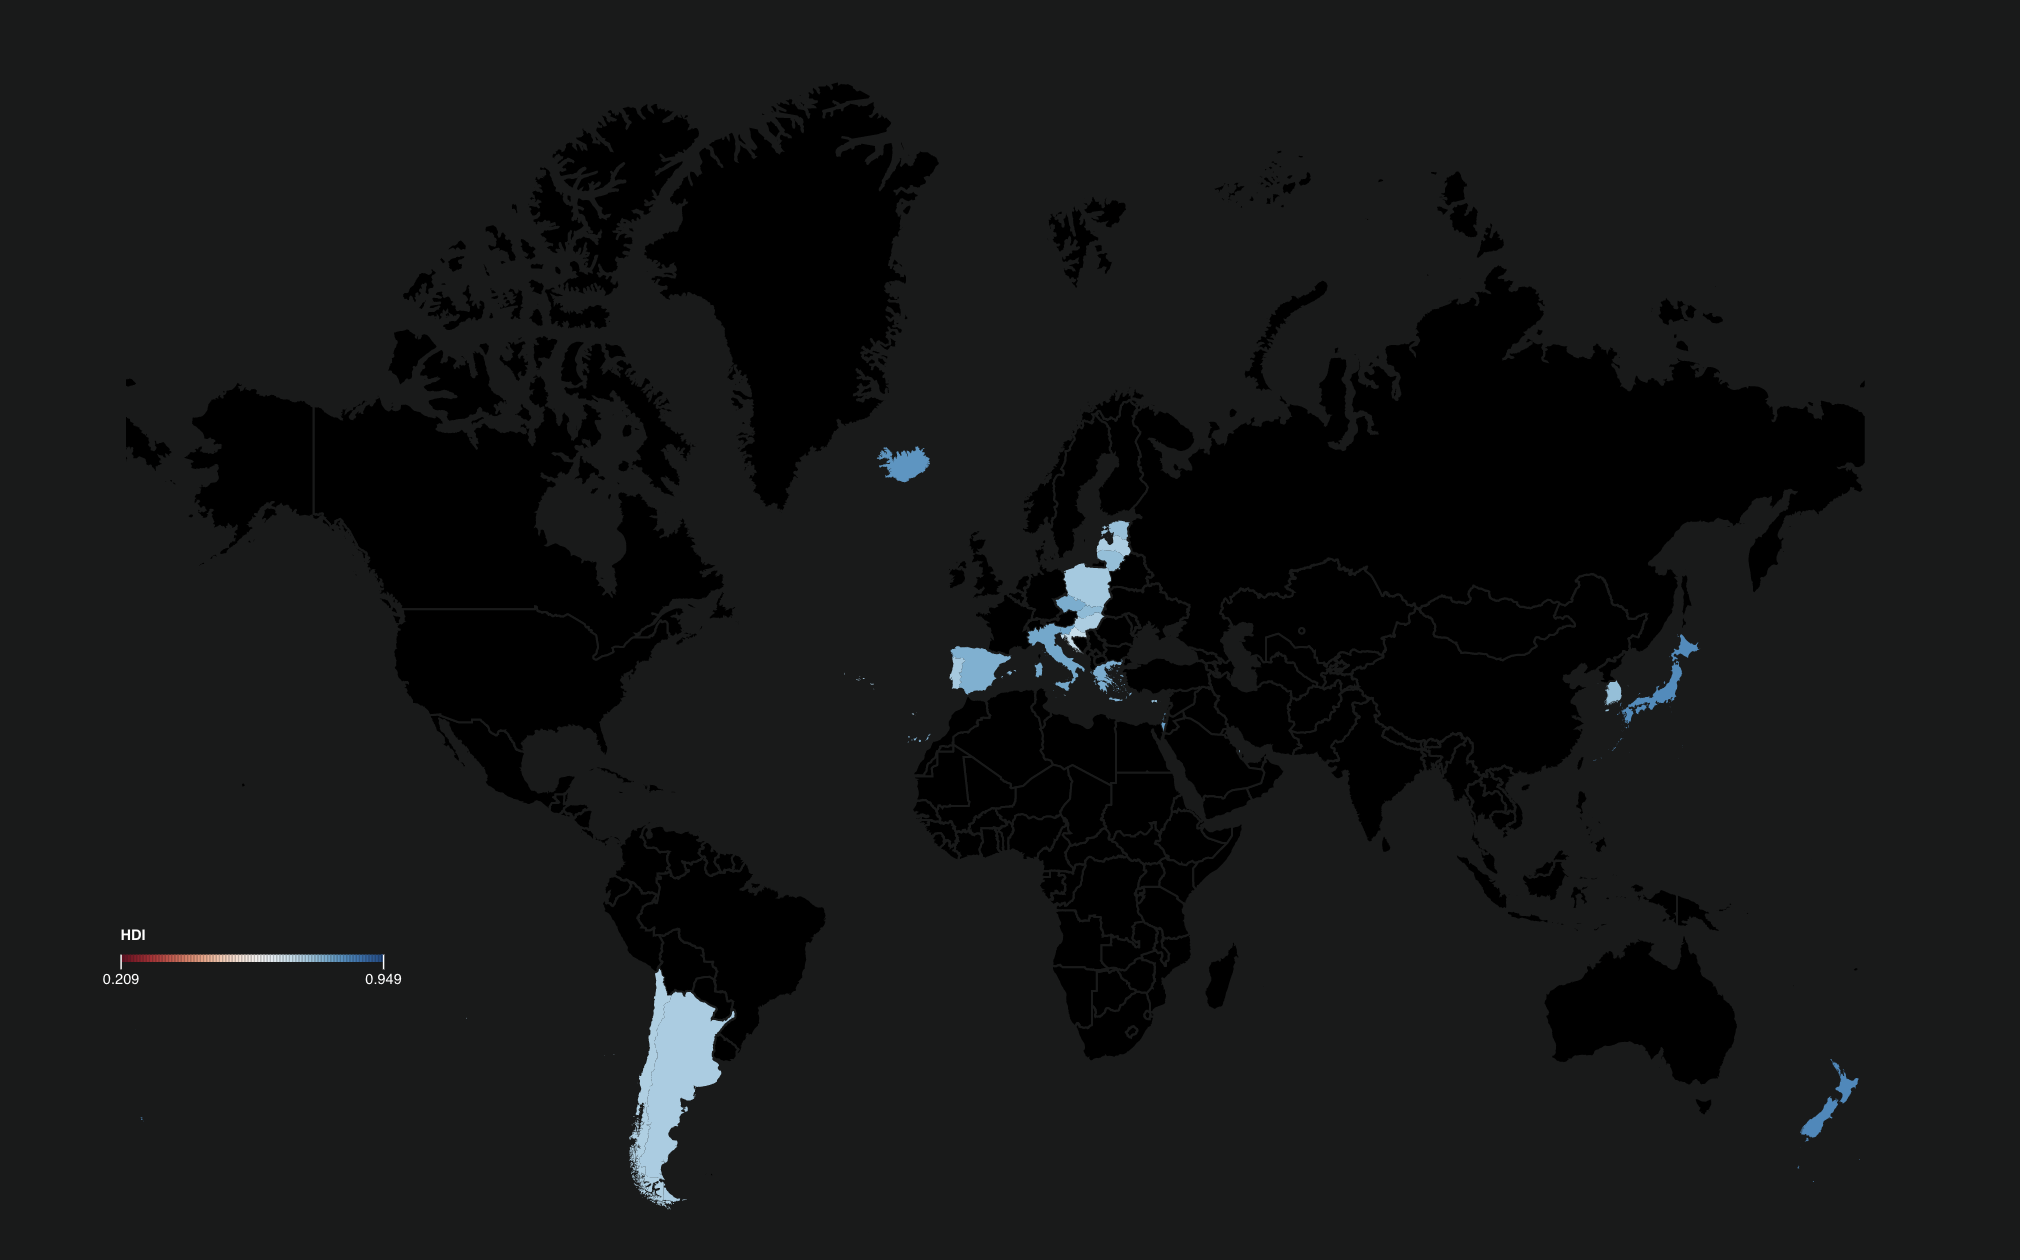
\includegraphics[width=0.4\textwidth]{filteredHdiMap}
		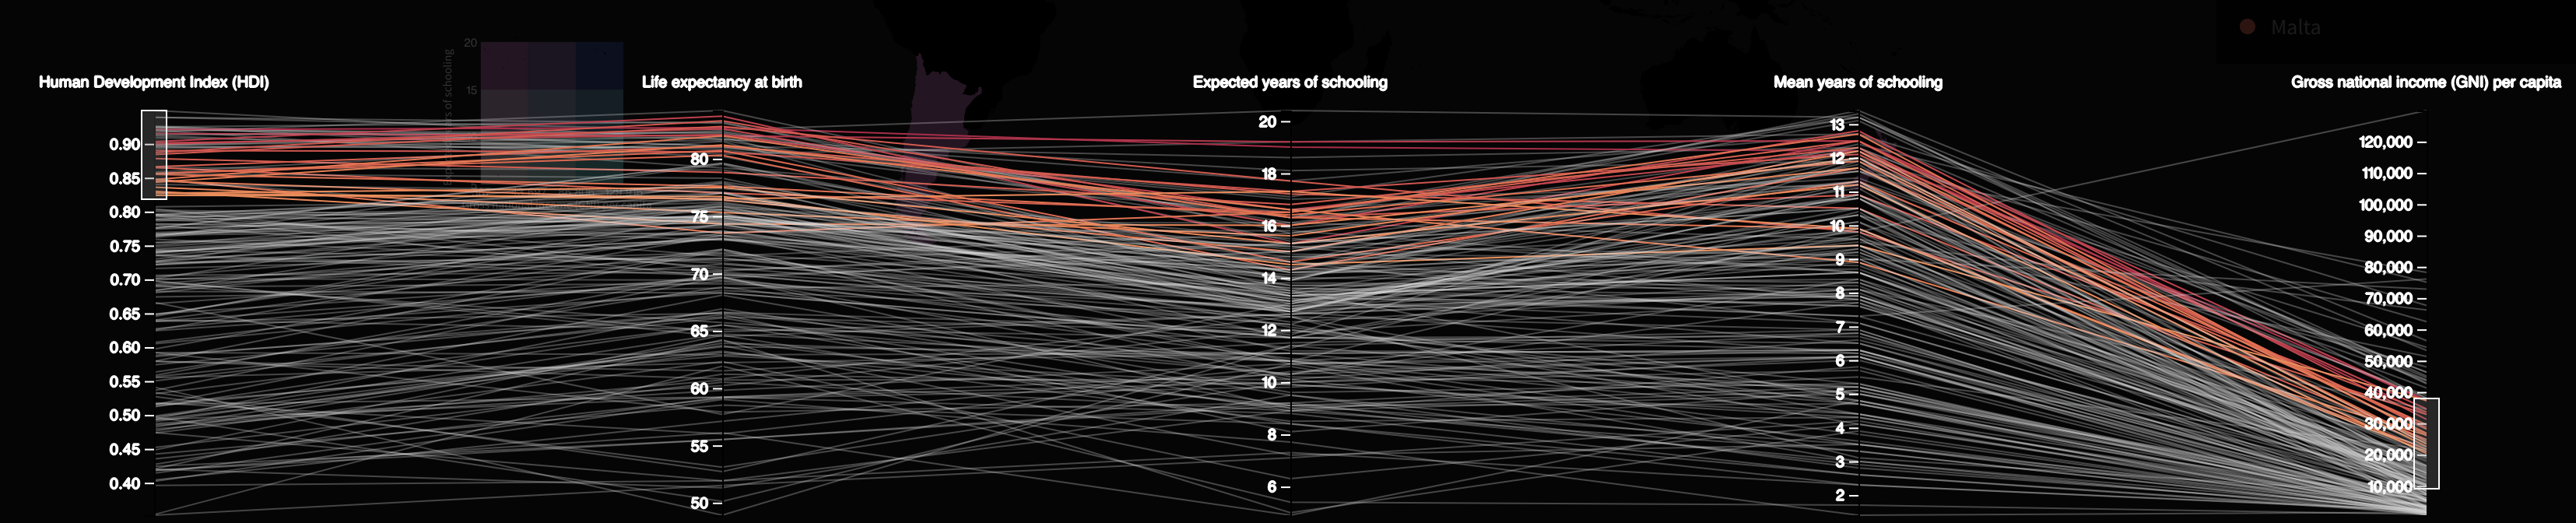
\includegraphics[width=0.4\textwidth]{parallelCoordGraph}
		\caption{Filter countries with high HDI and low GNI}
		\label{fig:parallel}
	\end{figure}
	\item \textbf{Controller:} there are three main components for the controller: map selector, year slider, and component selector. The map selector is responsible for selecting HDI Map Layer or Bivariate Map Layer to show. If HDI Map Layer is selected, the year slider will appear as well to allow users to slide between 1990 and 2015. Correspondingly, the HDI map will show the data from a specific year, which provides a historical view of the change in HDI over the years. If Bivariate Map Layer is selected, the year slider will be hidden and the component slider will be shown so that users can select which two components they are interested in (Figure~\ref{fig:controller}).
	\begin{figure}[t]
		\centering
        \subfloat[Select HDI map]{{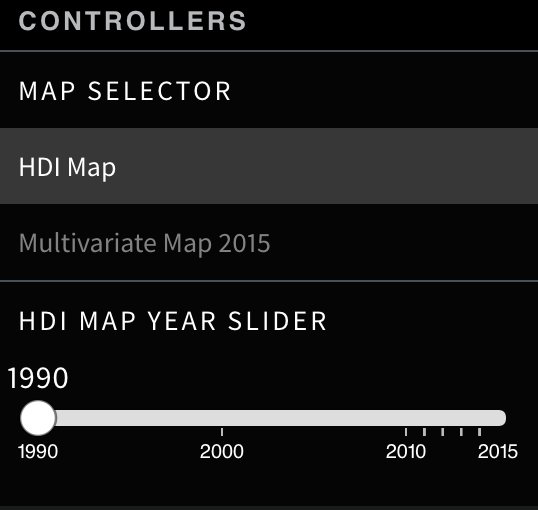
\includegraphics[width=3cm]{controllerHdi} }}%
        \qquad
        \subfloat[Select Bivariate Map]{{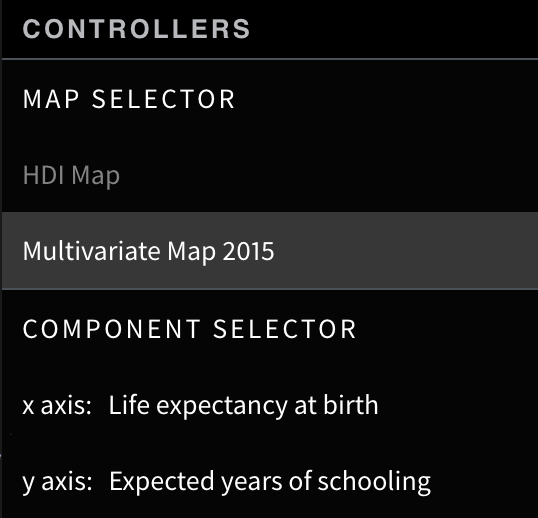
\includegraphics[width=3cm]{controllerBivariate} }}%
		\caption{Controller}
		\label{fig:controller}
	\end{figure}
    \item \textbf{Country Selector:} the country selector includes a search bar and a list of countries. The legend color next to each country name indicates the line color of the country shown in Parallel Coordinate Plot. The search bar allows users to select countries and helps user find a specific country on the world map. In additions, when users click on a country in the list, the corresponding country polygon on the world map and corresponding country line in the parallel coordinate plot will be highlighted. The detailed information of the country will be shown on the left side in Country Info Panel.
    \item \textbf{Country Info Panel:} the panel displays information about the country selected either from the map or from Country Selector. It contains two parts: statistics and a radar chart. \todo{add the figure and update ``xx'' $\rightarrow$} As shown in Figure xx, the radar chart provides a straightforward view of the percentiles of the HDI and its components of a selected country. It is easier for users to compare two countries from the radar chart than from simple texts, because the similarity of two countries can be captured by similar shapes (Figure~\ref{fig:panel}).
    \begin{figure}[t]
    	\centering
        \subfloat[New Zealand information]{{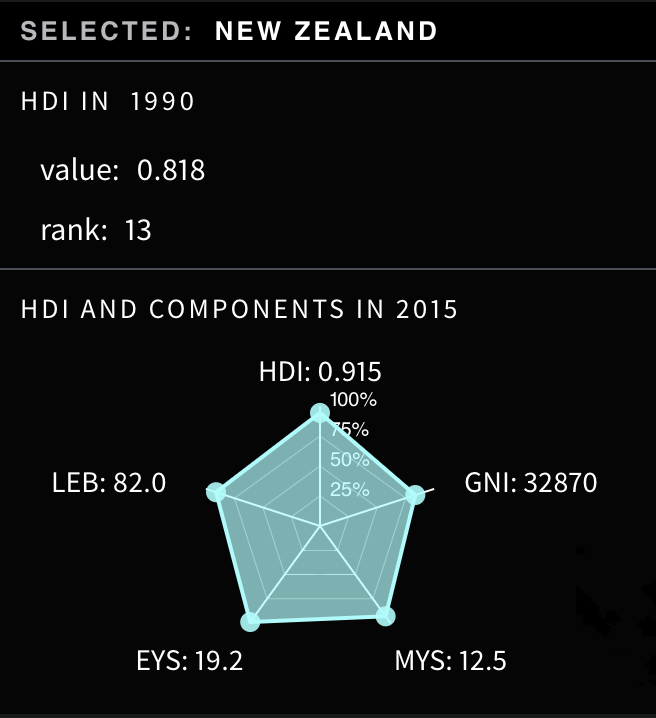
\includegraphics[width=3cm]{newZealand} }}%
        \qquad
        \subfloat[Korea information]{{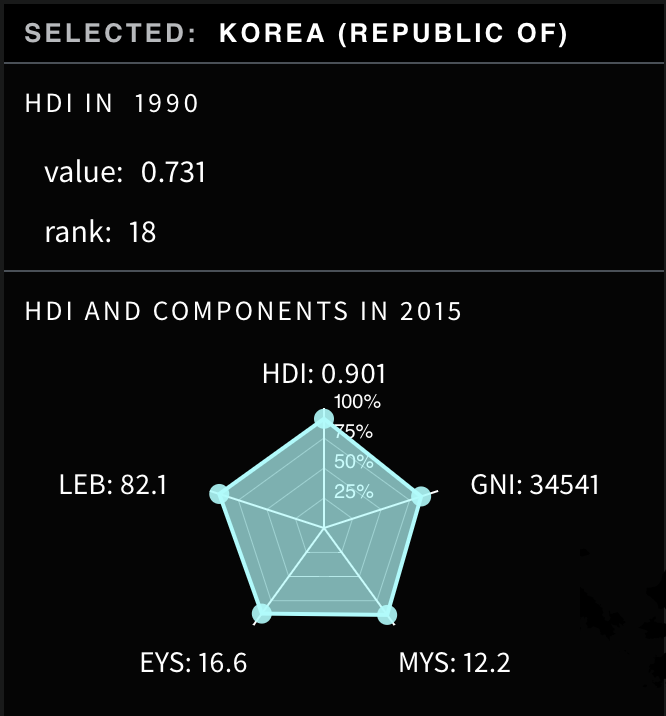
\includegraphics[width=3cm]{korea} }}%
    	\caption{New Zealand and Korea have close HDI ranks and values of HDI components}
    	\label{fig:panel}
    \end{figure}
\end{itemize}

\subsection{Design Logic}
To creating the preceding UI components, we have a main HTML file that includes one HTML \texttt{<div>} wrapper with a unique id for each UI component. Each UI component is implemented in a single JS file as module, where we extract the corresponding wrapper div from the main HTML file to build visualizations. For the charts and map, we use D3.js to create svg and inner layers. For communication between different UI components, we use d3.dispatch to generate event dispatchers and event listeners.  We also have a global JS file to shares global variables among all the components. As for styling, we create one CSS file for each component to independently set styles of components.
